\documentclass{article}
\usepackage{graphicx}
\usepackage{hyperref}
\usepackage{listings}
\usepackage{tcolorbox}
\usepackage{verbatim}
\usepackage{adjustbox}
\usepackage{float} % Add float package for better figure control

\title{Creating an EC2 Instance, SSH Access, and S3 Bucket on AWS}
\author{Priyanshu Kumar Sharma, 2022-B-17102004A, B.Tech CTIS, SEM-VI/B}
\date{\today}

\begin{document}

\maketitle

\section{Introduction}
This report details the step-by-step procedure for launching an EC2 instance on AWS, connecting to it via SSH, and creating an S3 bucket using Terraform. Screenshots are provided for better understanding.

\section{Creating an EC2 Instance on AWS Console}

\subsection{Step 1: Log in to AWS}
Go to \href{https://aws.amazon.com/}{AWS Management Console} and sign in.

\subsection{Step 2: Navigate to EC2 Dashboard}
From the AWS services, select \textbf{EC2}.

\subsection{Step 3: Launch a New Instance}
Click on \textbf{Launch Instance}.

\begin{figure}[H]
    \centering
    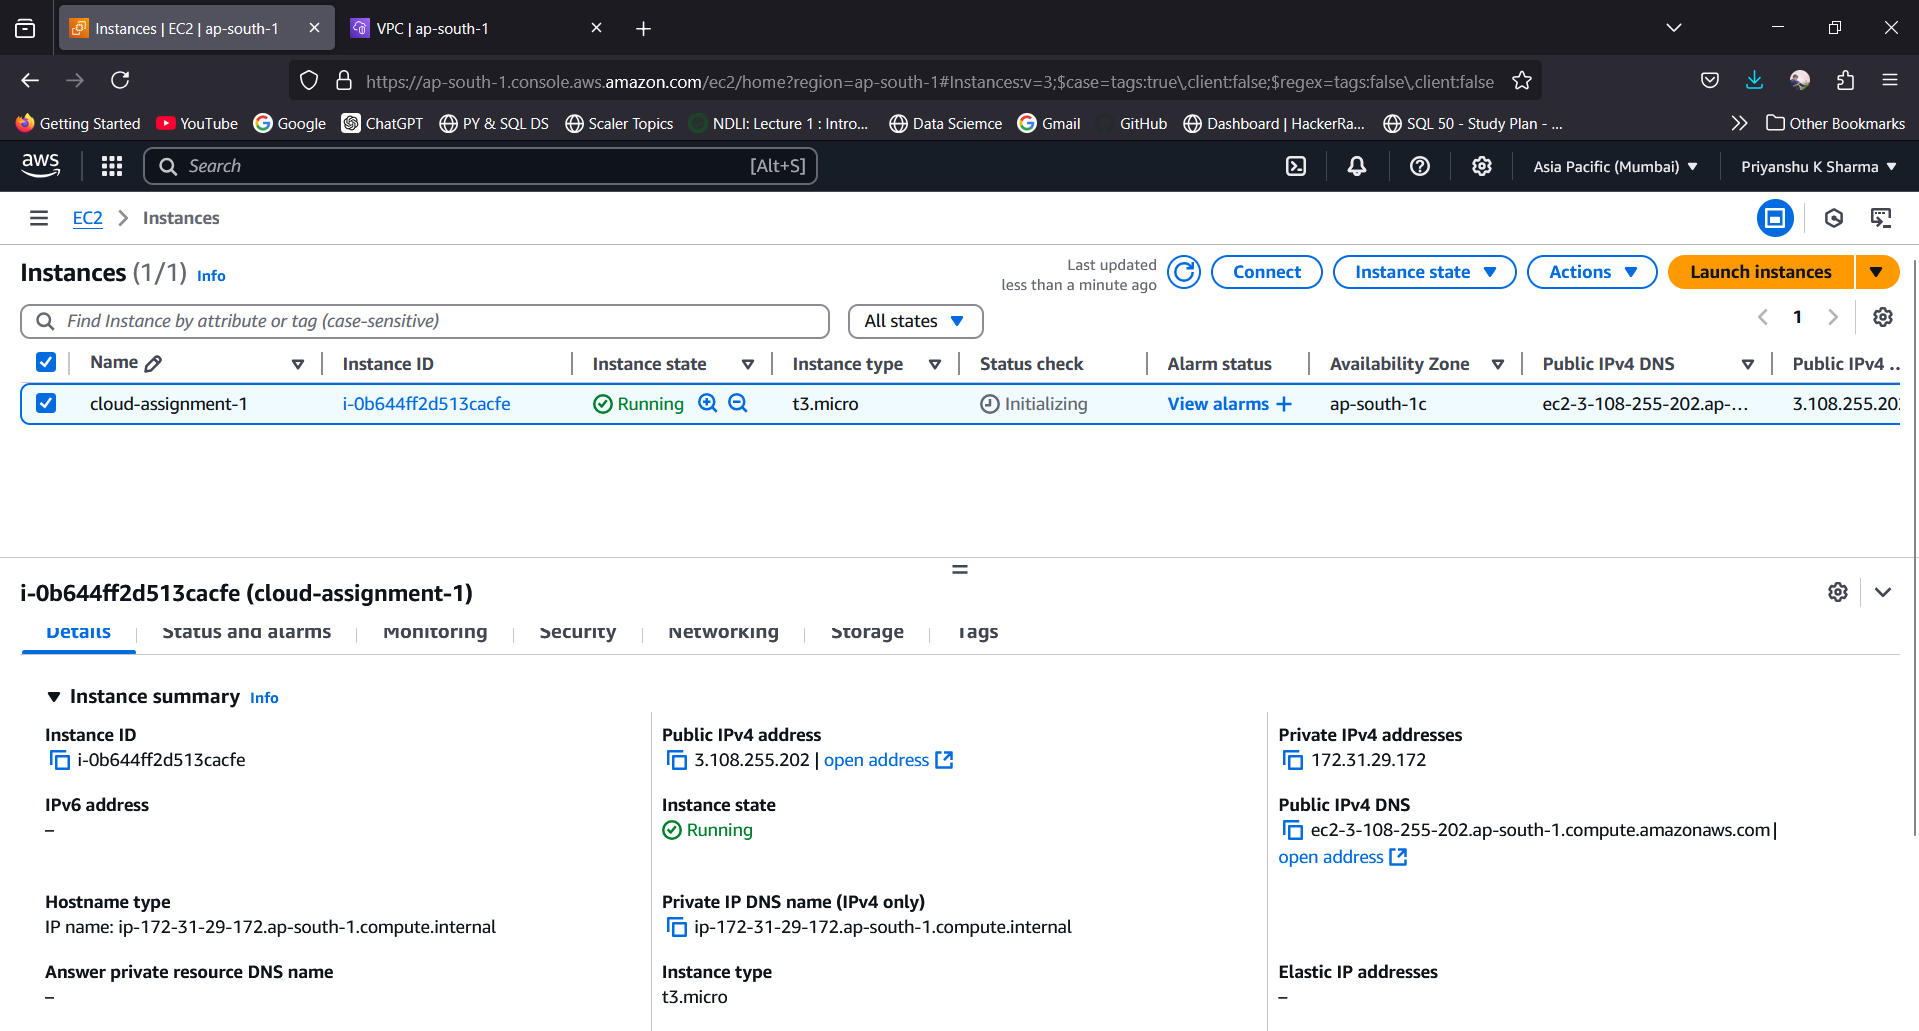
\includegraphics[width=\textwidth]{images/ec2_dashborad.png}
    \caption{EC2 Dashboard}
    \label{fig:ec2_dashboard}
\end{figure}

\subsection{Step 4: Configure Instance Details}
- Choose an AMI (e.g., Ubuntu 22.04 LTS).
- Select instance type (e.g., t2.micro).
- Configure security groups (allow SSH access from your IP).
- Assign a key pair for SSH access.

\begin{figure}[H]
    \centering
    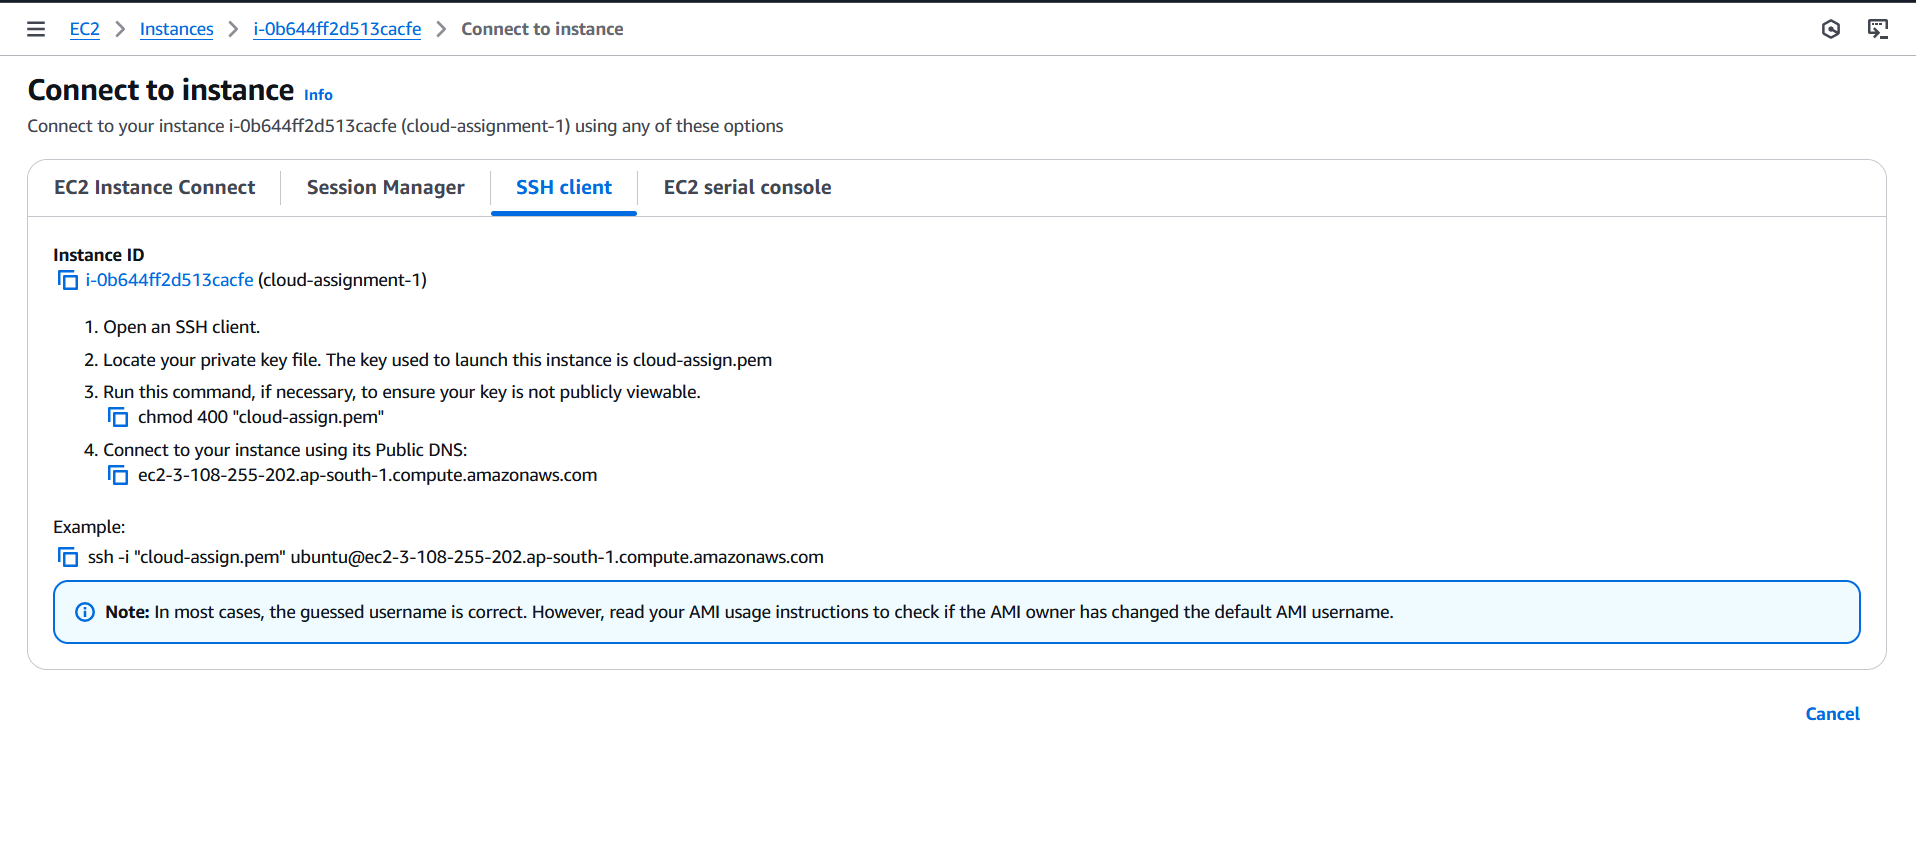
\includegraphics[width=\textwidth]{images/ec2-ssh.png}
    \caption{Connecting EC2 Instance with SSH}
    \label{fig:instance_ssh}
\end{figure}

\subsection{Step 5: Launch and Verify}
Click \textbf{Launch} and wait for the instance to initialize.

\section{Fixing SSH Private Key Permission Issues on Windows}

When connecting to an EC2 instance using SSH on Windows, you may encounter an error due to improper file permissions on your private key (.pem file). The necessary fixes and configurations are stored in a GitHub repository:

\href{https://github.com/itspriyanshuks17/EC2-Windows-Connect.git}{EC2 Windows SSH Connection Fix}

\subsection{Error Message Example}

\begin{tcolorbox}[colback=gray!10, colframe=black, title=Common Error]
\begin{adjustbox}{minipage=0.95\textwidth}
\begin{verbatim}
@@@@@@@@@@@@@@@@@@@@@@@@@@@@@@@@@@@@@@@@@@@@@@@@@@@@@@@@@@@
@         WARNING: UNPROTECTED PRIVATE KEY FILE!          @
@@@@@@@@@@@@@@@@@@@@@@@@@@@@@@@@@@@@@@@@@@@@@@@@@@@@@@@@@@@
Permissions for 'C:\path\to\your-key.pem' are too open.
It is required that your private key files are NOT 
accessible by others.
Load key "C:\path\to\your-key.pem": bad permissions
Permission denied (publickey).
\end{verbatim}
\end{adjustbox}
\end{tcolorbox}

\begin{figure}[H]
  \centering
  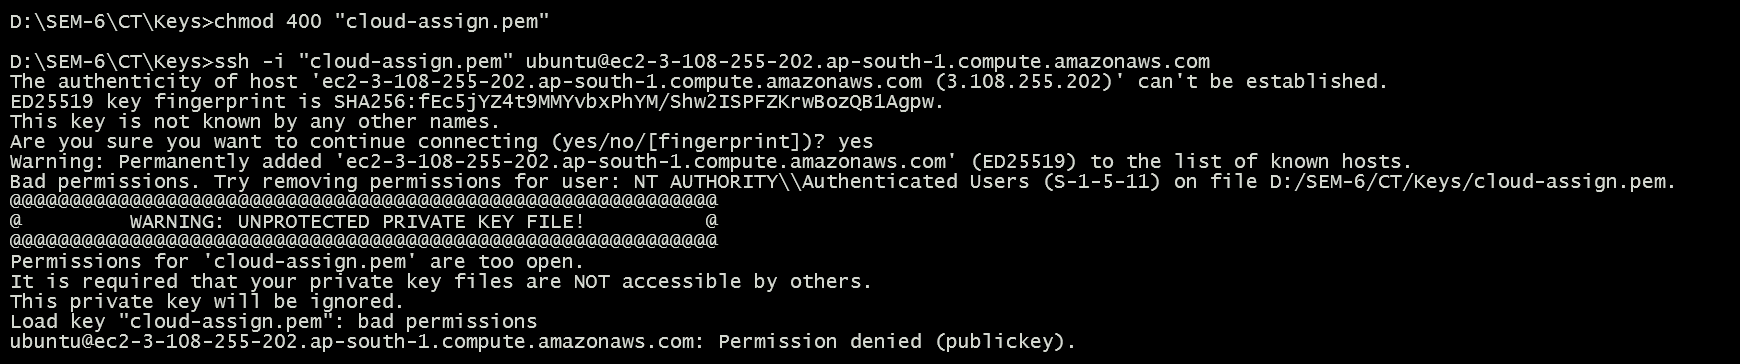
\includegraphics[height=04cm, width=13cm]{images/expected_error.png}
  \caption{Configuring EC2 Instance}
  \label{fig:Expected error}
\end{figure}



\subsection{Step 1: Open PowerShell as Administrator}
1. Press `Win + X` and select **PowerShell (Admin)**.
2. Navigate to the directory where your .pem file is stored:

\begin{tcolorbox}[colback=gray!10, colframe=black, title=Navigate to Key Folder]
cd "C://path//to//your-key-folder"
\end{tcolorbox}

\subsection{Step 2: Fix Key File Permissions}
Run the following commands in PowerShell:

\begin{tcolorbox}[colback=gray!10, colframe=black, title=Remove Inherited Permissions]
icacls "your-key.pem" /inheritance:r
\end{tcolorbox}

\begin{tcolorbox}[colback=gray!10, colframe=black, title=Remove Unauthorized Users]
icacls "your-key.pem" /remove "Authenticated Users" "Everyone" "BUILTIN\\Users"
\end{tcolorbox}

\begin{tcolorbox}[colback=gray!10, colframe=black, title=Grant Read-Only Access to Current User]
icacls "your-key.pem" /grant:r "%USERNAME%:R"
\end{tcolorbox}

\subsection{Step 3: Verify Correct Permissions}

\begin{tcolorbox}[colback=gray!10, colframe=black, title=Check Key File Permissions]
icacls "your-key.pem"
\end{tcolorbox}

Output should look like:
your-key.pem YOUR-PC\YourUsername:(R)

\begin{figure}[h]
  \centering
  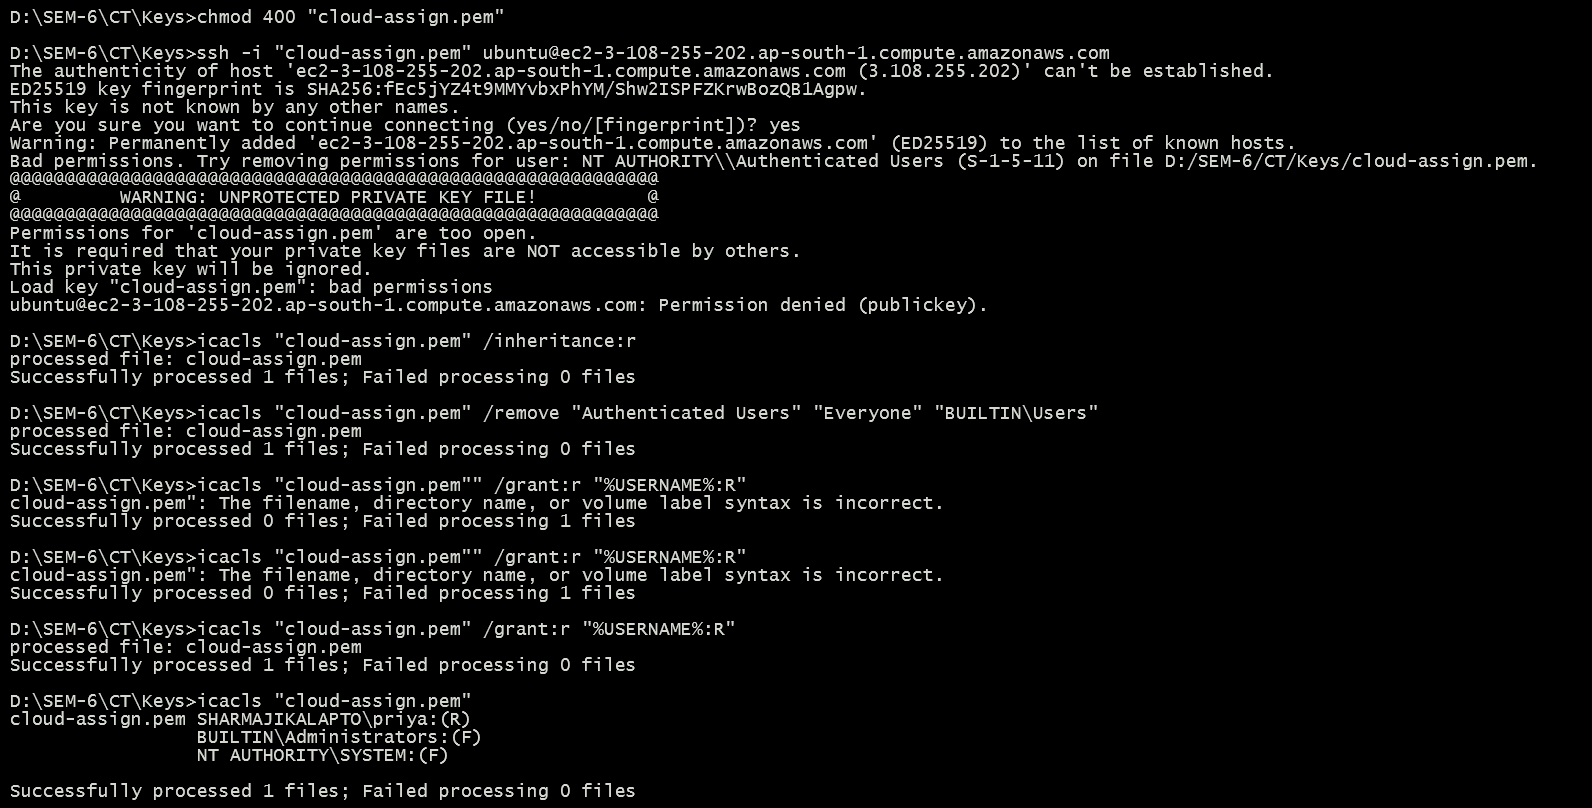
\includegraphics[height=07cm, width=10cm]{images/error_fixing.png}
  \caption{Error Fixing SSH}
  \label{fig:ssh connect-fix}
\end{figure}


\subsection{Step 4: Attempt SSH Connection Again}

\begin{tcolorbox}[colback=gray!10, colframe=black, title=SSH Command]
ssh -i "C://path//to//your-key.pem" ubuntu@your-ec2-instance.amazonaws.com
\end{tcolorbox}

\begin{figure}[h]
  \centering
  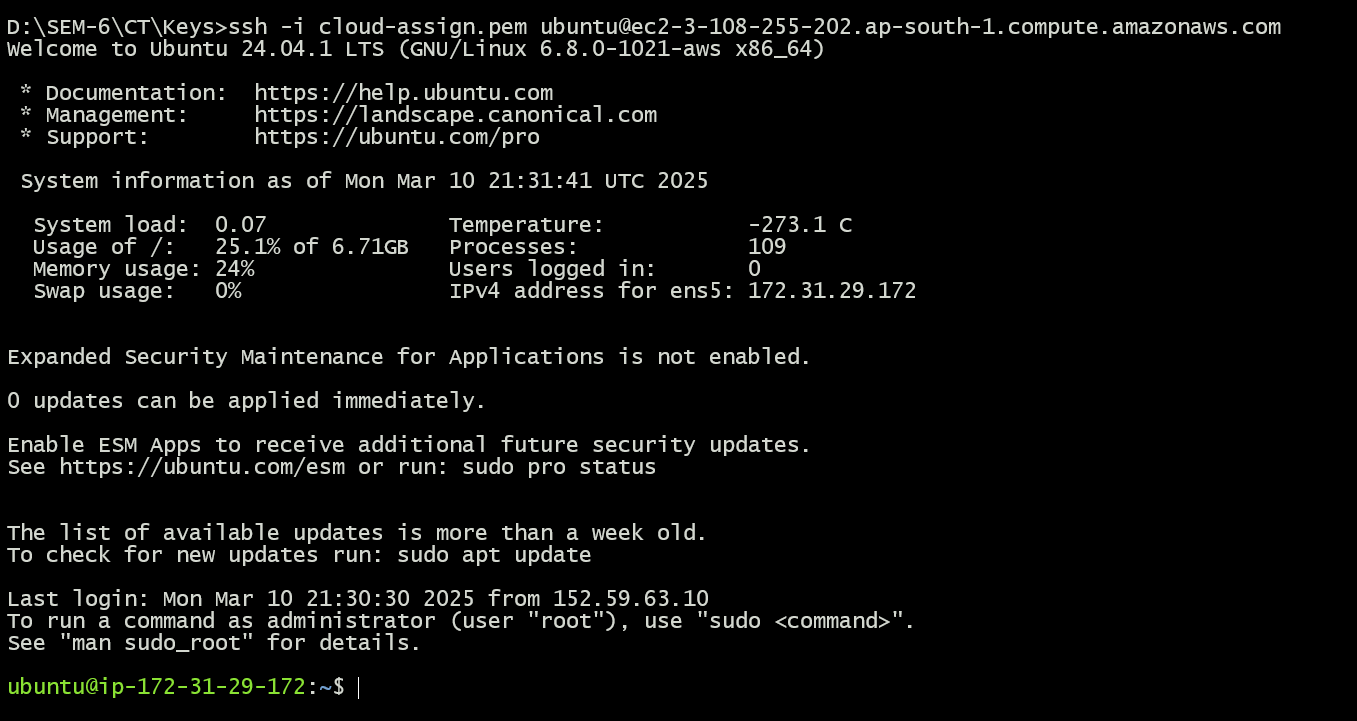
\includegraphics[height=06cm, width=10cm]{images/ssh_connect.png}
  \caption{SSH Connect Windows}
  \label{fig:ssh connect}
\end{figure}

% Add this section before the Conclusion section

\section{Creating an S3 Bucket Using Terraform}

\subsection{Step 1: Install Terraform (If Not Installed)}
Run the following commands:

\begin{tcolorbox}[colback=gray!10, colframe=black, title=Install Terraform]
sudo apt update && sudo apt install -y terraform
terraform --version
\end{tcolorbox}

Ensure AWS credentials are configured:

\begin{tcolorbox}[colback=gray!10, colframe=black, title=Configure AWS CLI]
aws configure
\end{tcolorbox}

\begin{figure}[H]
  \centering
  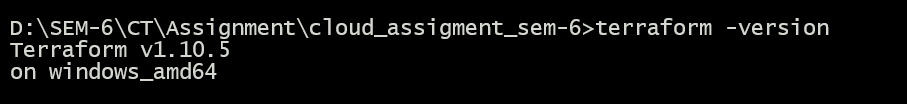
\includegraphics[width=1\textwidth]{images/terraform_install.png}
  \caption{Installing Terraform and Configuring AWS CLI}
  \label{fig:terraform_install}
\end{figure}

\subsection{Step 2: Create Terraform Configuration Files}

\subsubsection{Create a Terraform Directory}

\begin{tcolorbox}[colback=gray!10, colframe=black, title=Create Directory]
mkdir terraform-s3 && cd terraform-s3
\end{tcolorbox}

\subsubsection{Create the \texttt{main.tf} File}

Create a new file named \texttt{main.tf} and add the following Terraform configuration:

\begin{tcolorbox}[colback=gray!10, colframe=black, title=Terraform Configuration]
\begin{verbatim}
provider "aws" {
  region = "us-east-1"
}

resource "aws_s3_bucket" "cloud_assignment_bucket" {
  bucket = "cloud-assignment-bucket-1710"
}
\end{verbatim}
\end{tcolorbox}

\begin{tcolorbox}[colback=gray!10, colframe=black, title=Uploading file to S3]
  \begin{verbatim}
    resource "aws_s3_object" "example_file" {
      bucket = aws_s3_bucket.cloud_assignment_bucket.id
      key    = "uploaded-file.txt"
      source = "./uploaded-file.txt"
      acl    = "private"
    }
  \end{verbatim}
  \end{tcolorbox}

\subsection{Step 3: Initialize and Apply Terraform Configuration}

\begin{tcolorbox}[colback=gray!10, colframe=black, title=Initialize Terraform]
terraform init
\end{tcolorbox}

\begin{figure}[H]
  \centering
  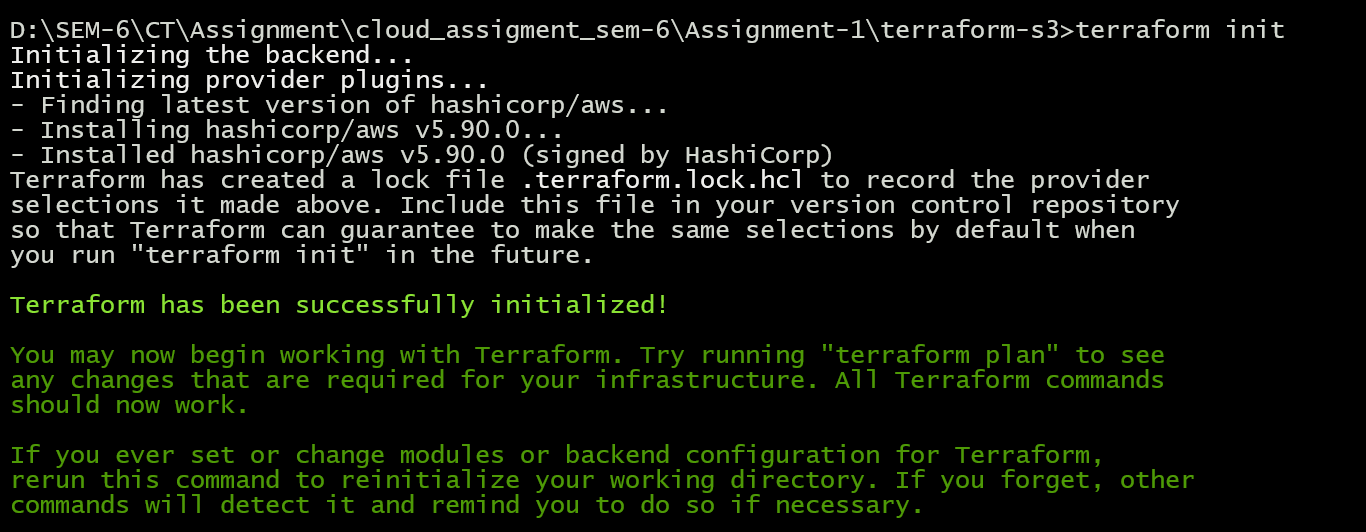
\includegraphics[width=0.9\textwidth]{images/terraform_init.png}
  \caption{Creating Terraform Configuration Files}
  \label{fig:terraform_config}
\end{figure}


\begin{tcolorbox}[colback=gray!10, colframe=black, title=Validate Terraform Configuration]
terraform validate
\end{tcolorbox}

\begin{tcolorbox}[colback=gray!10, colframe=black, title=Apply Terraform Configuration]
terraform apply -auto-approve
\end{tcolorbox}

\begin{figure}[H]
  \centering
  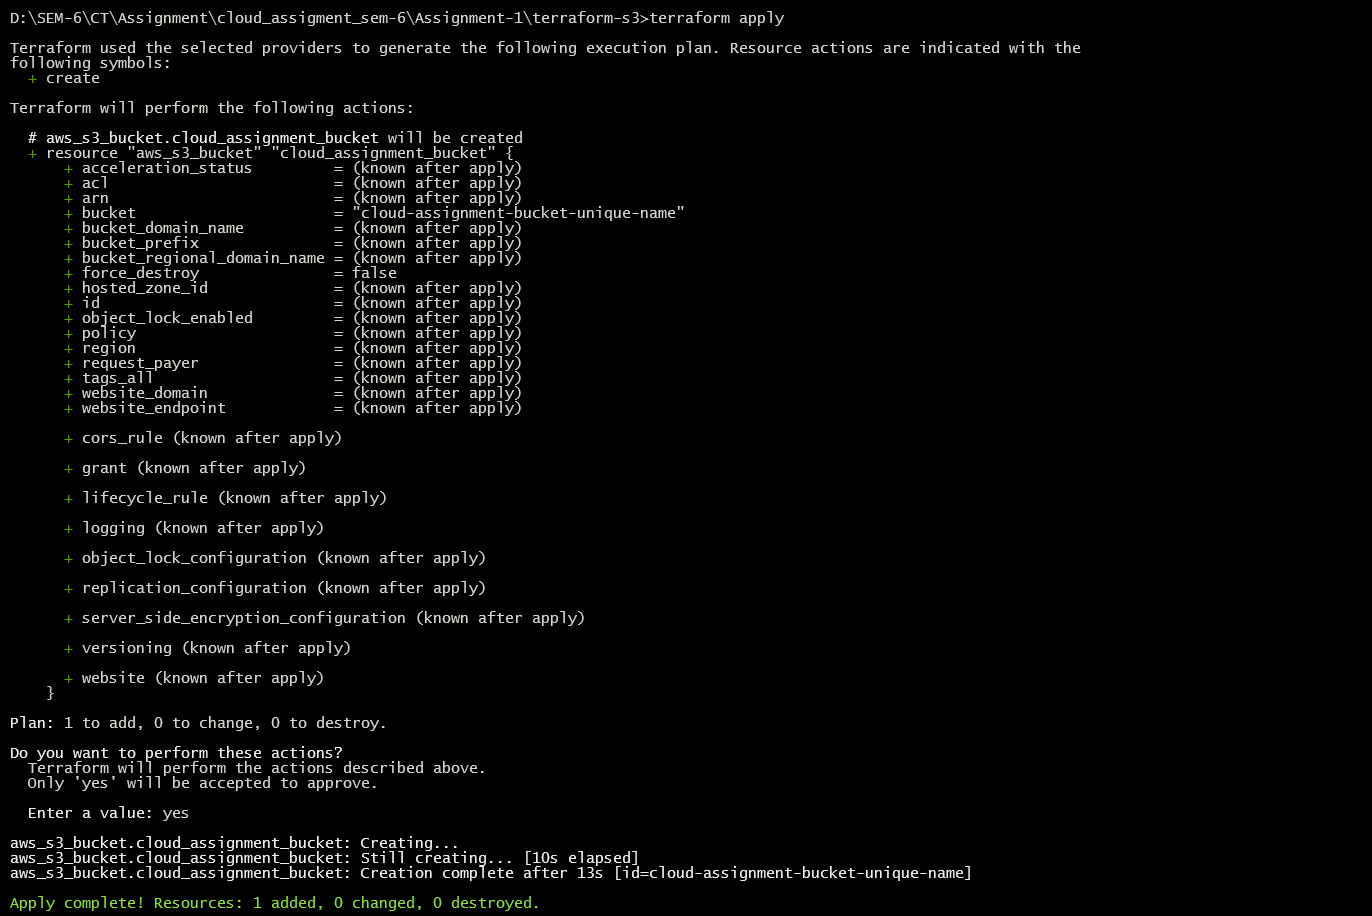
\includegraphics[width=0.9\textwidth]{images/terraform_apply.png}
  \caption{Initializing and Applying Terraform Configuration}
  \label{fig:terraform_apply}
\end{figure}

\newpage

\subsection{Step 4: Verify S3 Bucket Creation}

After successful execution, verify the bucket creation in AWS Console.

\begin{figure}[H]
  \centering
  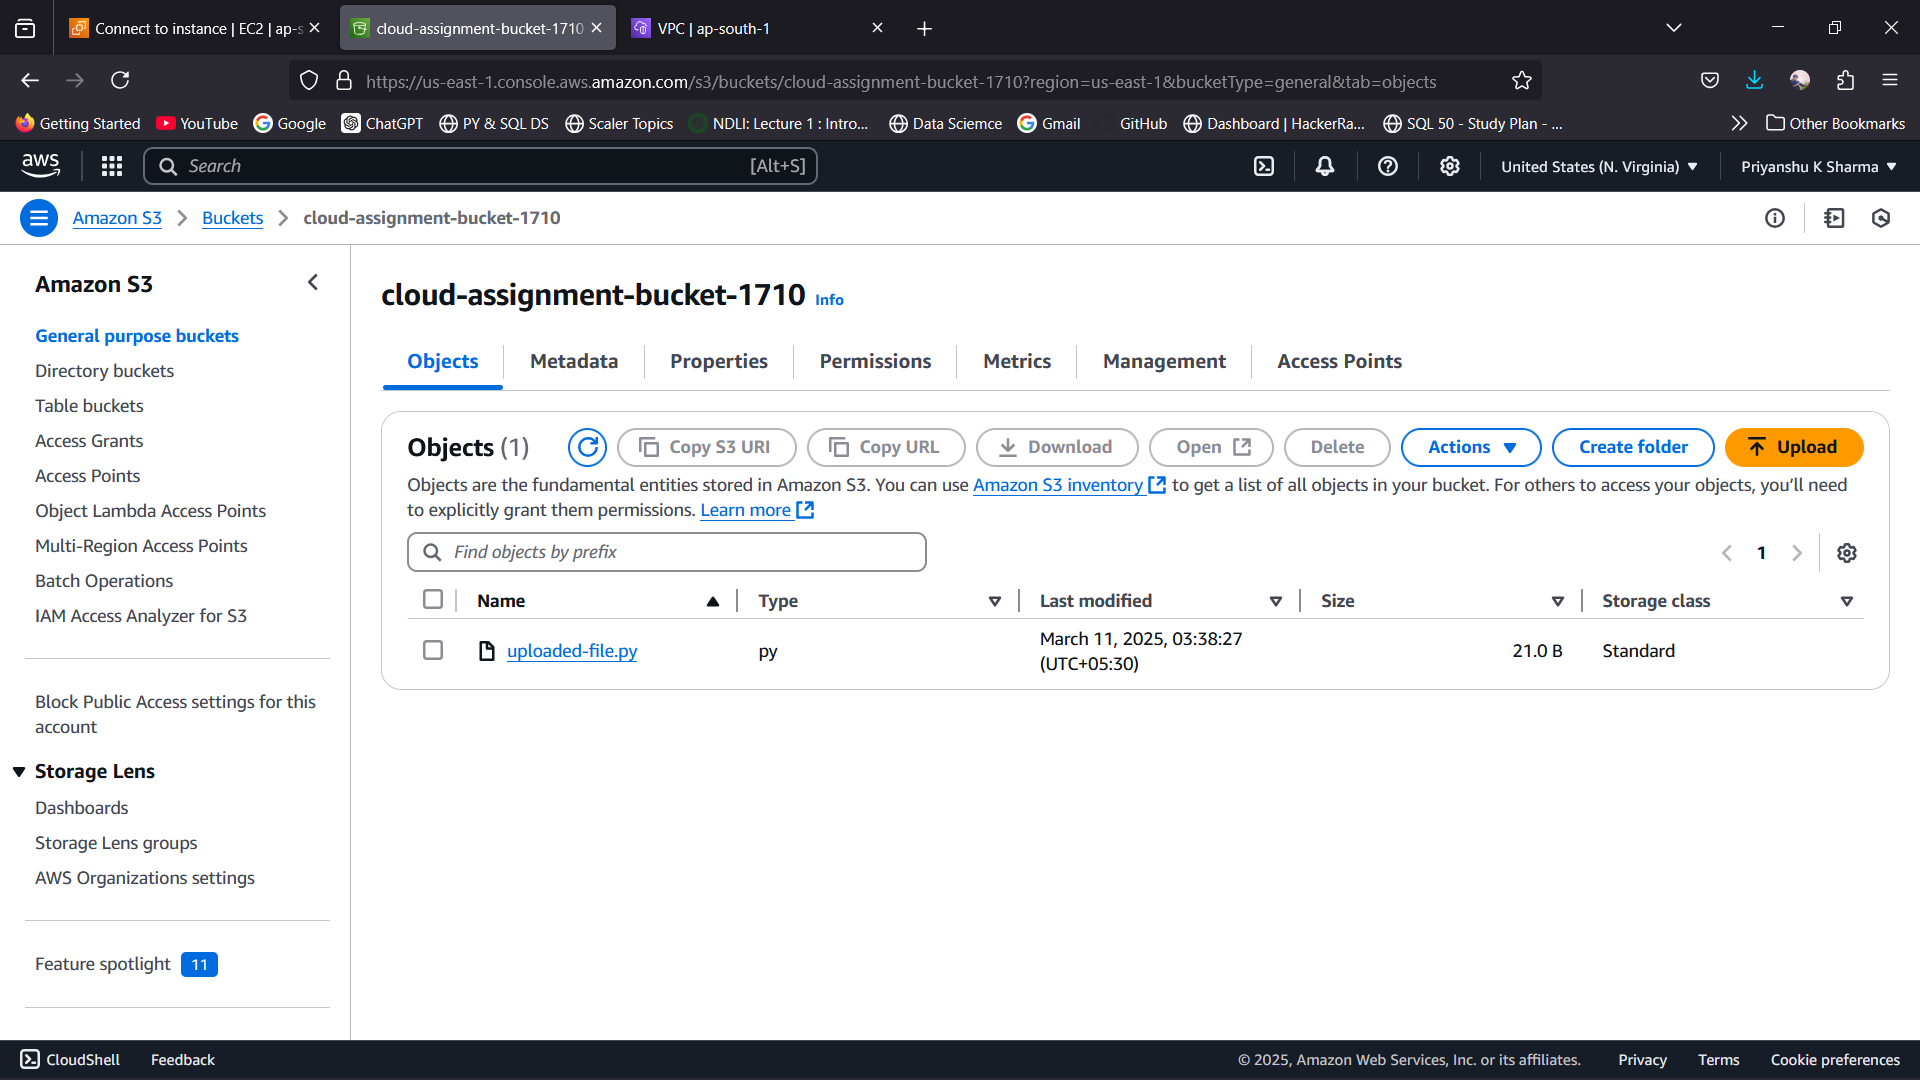
\includegraphics[width=0.9\textwidth]{images/s3_bucket_created.png}
  \caption{S3 Bucket Created Successfully}
  \label{fig:s3_bucket}
\end{figure}

\section{Conclusion}
This report covered the process of launching an EC2 instance, fixing SSH private key permissions on Windows, and setting up an S3 bucket using Terraform. These are fundamental cloud operations useful in AWS environments.

\end{document}
